\documentclass[runningheads,a4paper,11pt]{report}

\usepackage{algorithmic}
\usepackage{algorithm} 
\usepackage{array}
\usepackage{amsmath}
\usepackage{amsfonts}
\usepackage{amssymb}
\usepackage{amsthm}
\usepackage{caption}
\usepackage{comment} 
\usepackage{epsfig} 
\usepackage{fancyhdr}
\usepackage[T1]{fontenc}
\usepackage{geometry} 
\usepackage{graphicx}
\usepackage[colorlinks]{hyperref} 
\usepackage[latin1]{inputenc}
\usepackage{multicol}
\usepackage{multirow} 
\usepackage{rotating}
\usepackage{setspace}
\usepackage{subfigure}
\usepackage{url}
\usepackage{verbatim}
\usepackage{xcolor}
\usepackage[romanian]{babel}

\geometry{a4paper,top=3cm,left=2cm,right=2cm,bottom=3cm}

\pagestyle{fancy}
\fancyhf{}
\fancyhead[LE,RO]{Reconstituiri istorice}
\fancyfoot[RE,LO]{MIRPR 2021-2022}
\fancyfoot[LE,RO]{\thepage}

\renewcommand{\headrulewidth}{2pt}
\renewcommand{\footrulewidth}{1pt}
\renewcommand{\headrule}{\hbox to\headwidth{%
  \color{gray}\leaders\hrule height \headrulewidth\hfill}}
\renewcommand{\footrule}{\hbox to\headwidth{%
  \color{gray}\leaders\hrule height \footrulewidth\hfill}}

\hypersetup{
pdftitle={artTitle},
pdfauthor={name},
pdfkeywords={pdf, latex, tex, ps2pdf, dvipdfm, pdflatex},
bookmarksnumbered,
pdfstartview={FitH},
urlcolor=cyan,
colorlinks=true,
linkcolor=blue,
citecolor=blue,
}
% \pagestyle{plain}

\setcounter{secnumdepth}{3}
\setcounter{tocdepth}{3}

\linespread{1}

% \pagestyle{myheadings}

\makeindex


\begin{document}

\begin{titlepage}
\sloppy

\begin{center}
UNIVERSITATEA BABES BOLYAI, CLUJ NAPOCA, ROMANIA
\end{center}

\begin{center}
FACULTATEA DE MATEMATICA SI INFORMATICA
\end{center}

\begin{center}
\vspace{6cm}

\Huge \textbf{Reconstituiri istorice}

\vspace{1cm}

\normalsize -- MIRPR  --

\end{center}


\vspace{5cm}

\begin{flushright}
\Large{\textbf{Membrii echipei}}
\end{flushright}

\begin{flushright}
Andrei-Danut Blagoi, Informatica romana, grupa 231
\end{flushright}

\begin{flushright}
Andreea Bolonyi, Informatica romana, grupa 231
\end{flushright}

\begin{flushright}
Stefan-Nicolae Parvanescu, Informatica engleza, grupa 936
\end{flushright}

\begin{flushright}
Oana-Alexandra Sidorencu, Informatica romana, grupa 236
\end{flushright}

\vspace{4cm}

\begin{center}
2021-2022
\end{center}

\end{titlepage}

\pagenumbering{gobble}

\begin{abstract}
Proiectul propus este menit sa vina in ajutorul persoanelor pasionate de istorie si arheologie care isi doresc informatii plastice despre anumite date introduse. Utilizatorii aplicatiei au posibilitatea sa exploreze niste date numerice pe care le gasesc, reusind sa cunoasca care este sexul sau varsta unui os pe care acestia il studiaza si, de asemenea, utilizatorii au posibilitatea sa perceapa informatia si intr-un mod vizual.
\end{abstract}

\begin{figure}
\centerline{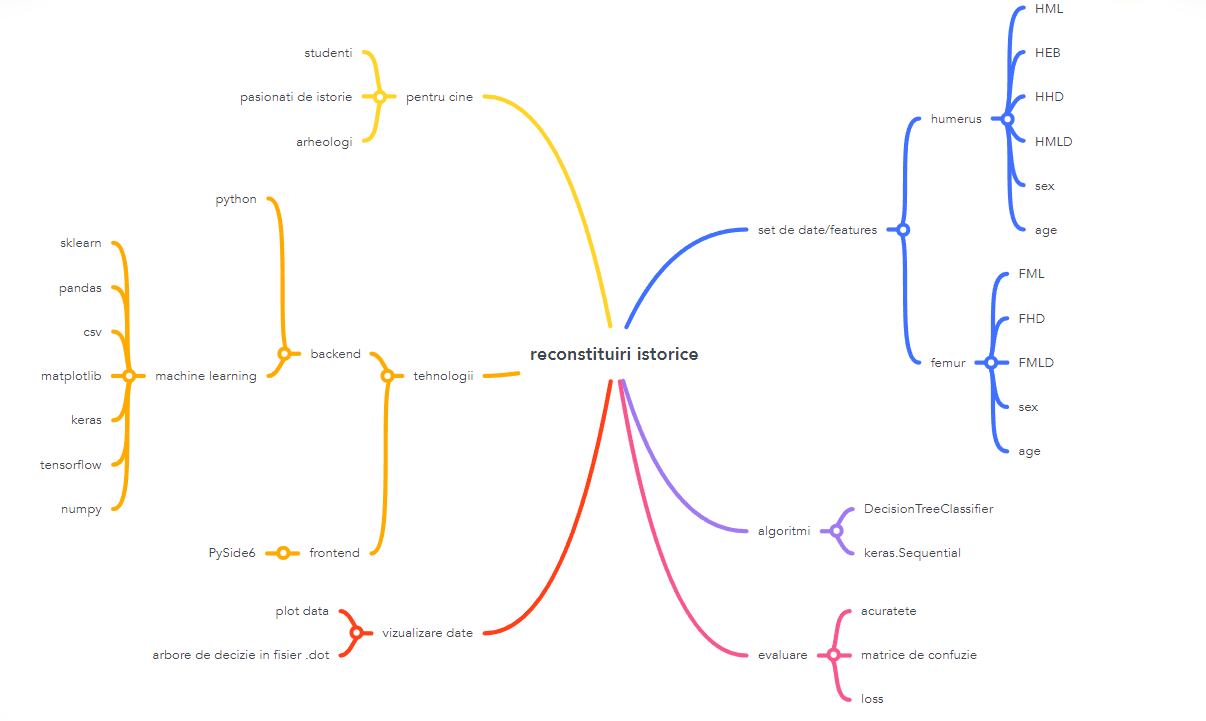
\includegraphics[width=23cm]{Imagini/mind-map.PNG}}
\caption{Mind map.}
\label{fig}
\end{figure}

\begin{figure}
\centerline{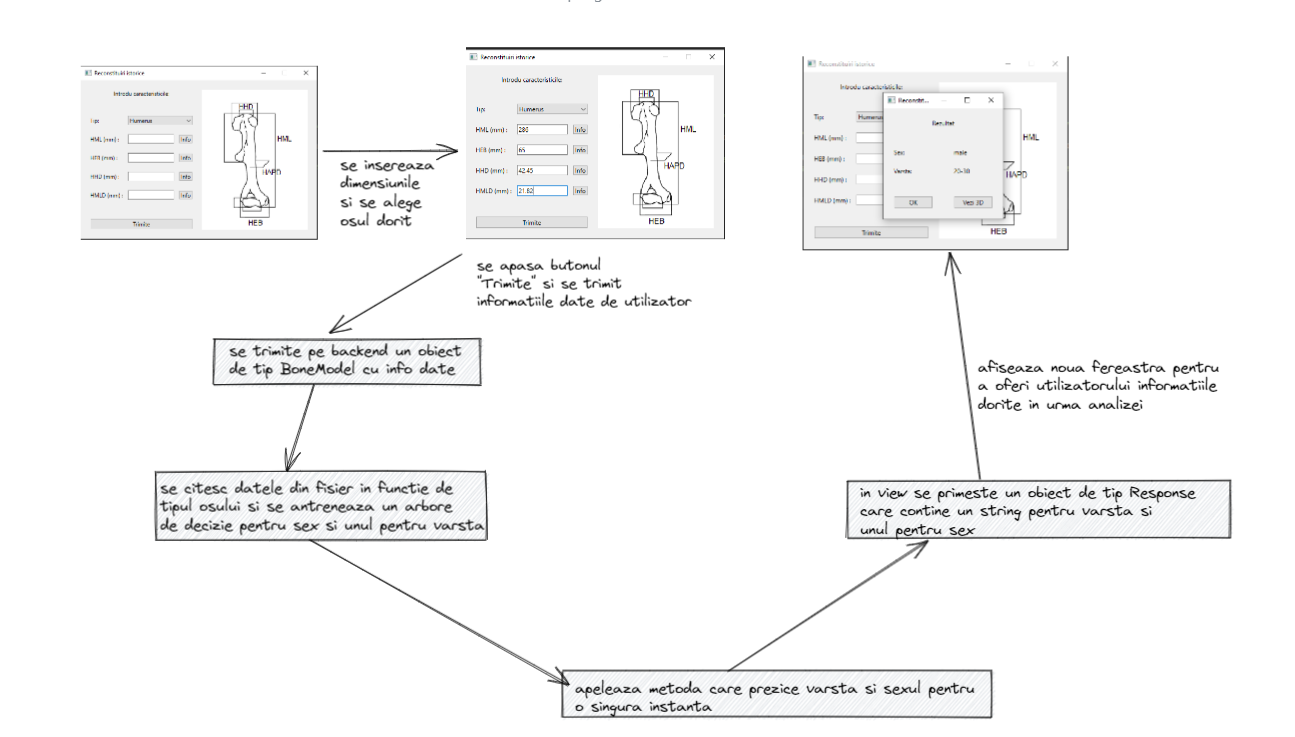
\includegraphics[width=22cm,height=15cm]{Imagini/flow.PNG}}
\caption{Flow al aplicatiei.}
\label{fig}
\end{figure}

\begin{figure}[h!]
\centerline{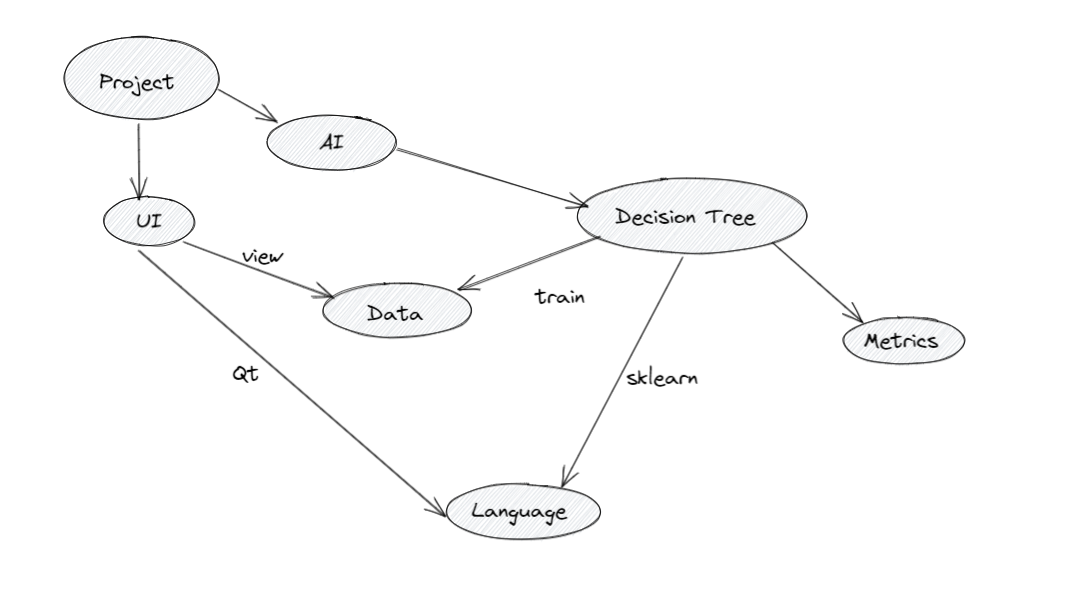
\includegraphics[width=22cm,height=10cm]{Imagini/ontology_decision_tree.PNG}}
\caption{Ontologia pentru arborele de decizie.}
\label{fig}
\end{figure}

\begin{figure}[h!]
\centerline{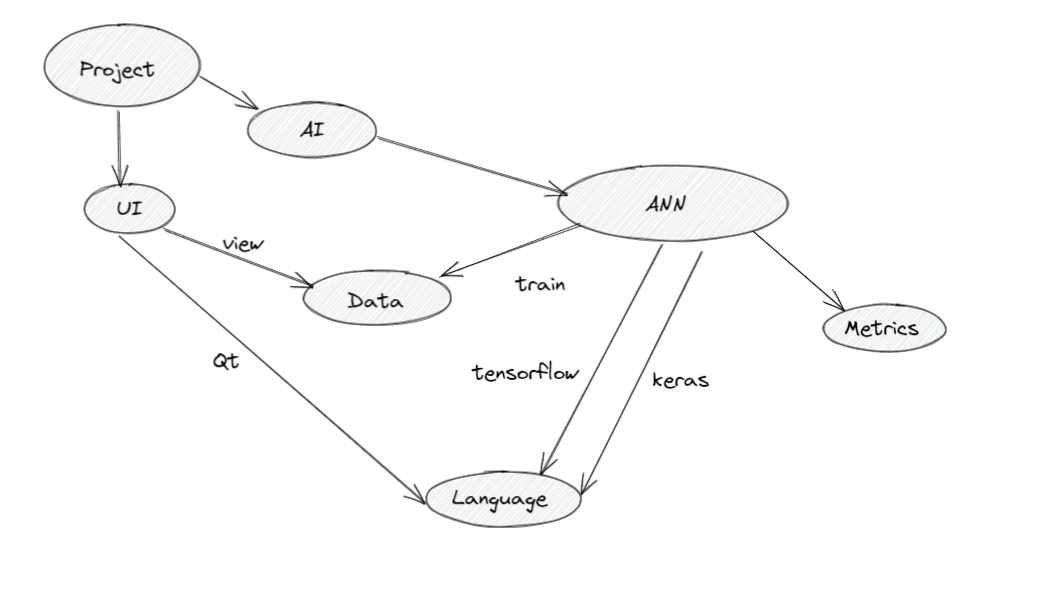
\includegraphics[width=22cm,height=10cm]{Imagini/ontology_ann.PNG}}
\caption{Ontologia pentru reteaua neuronala.}
\label{fig}
\end{figure}

\tableofcontents

\setstretch{1.5}

\newpage

\pagenumbering{arabic}

\chapter{Introducere}
\label{chapter:introducere}

\section{Motivarea temei}
\label{section:motivare}

Problema abordata in acest proiect este de interes pentru persoanele care lucreaza in acest domeniu, studenti ce vor ajunge angajati sau persoane care sunt doar pasionate. Aplicatia dezvoltata este usor de folosit, intuitiva si menita sa ofere doar ajutor, nu probleme utilizatorului. \newline \newline
Pasionatii folosind aplicatia noastra vor putea sa aiba o idee mult mai aprofundata in legatura cu subiectul pe care il studiaza, nu doar sa se bazeze pe niste cifre pe care le vad. De asemenea, o functionalitate pe care dorim sa o oferim utilizatorului este posibilitatea de a vedea 3D aceste informatii pe care le introduce. \newline

\section{Tehnologii}
\label{section:tehnologii}
Dezvoltarea aplicartiei se bazeaza pe limbajul Python pentru partea de backend si PyQT pentru partea de frontend. Am decis sa folosim Python datorita usurintei cu care se poate scrie codul si multitudinea de solutii pe care le putem gasi, fie ca este vorba de o problema obisnuita pentru un programator, fie ca este vorba de biblioteci din domeniul inteligentei artificiale pe care le putem folosi pentru rezolvarea subiectului (spre exemplu Scikit-learn, TensorFlow, Theano).

\section{Masuratori ale oaselor}
\label{section:masuratori}
Caracteristicile folosite pentru fiecare tip de os si semnificatiile lor.

\begin{figure}[h!]
\centerline{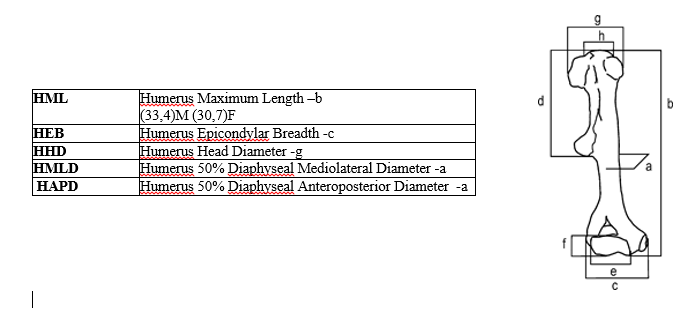
\includegraphics[height=10cm]{Imagini/humerus.PNG}}
\caption{Caracteristici humerus.}
\label{fig}
\end{figure}

\begin{figure}[h!]
\centerline{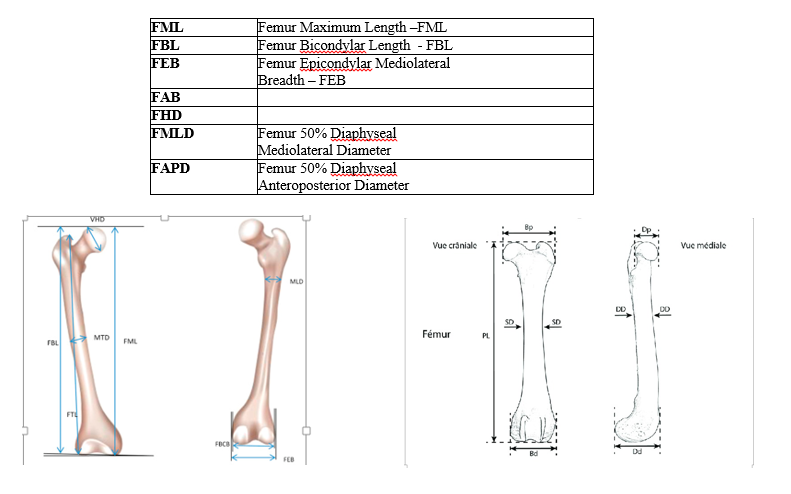
\includegraphics[height=10cm]{Imagini/femur.PNG}}
\caption{Caracteristici femur.}
\label{fig}
\end{figure}

\section{Setul de date}
\label{section:date}
Setul de date cu care s-a lucrat pentru fiecare tip de os (reprezentare grafica a numarului de elemente din fiecare categorie).

\begin{figure}[h!]
\centerline{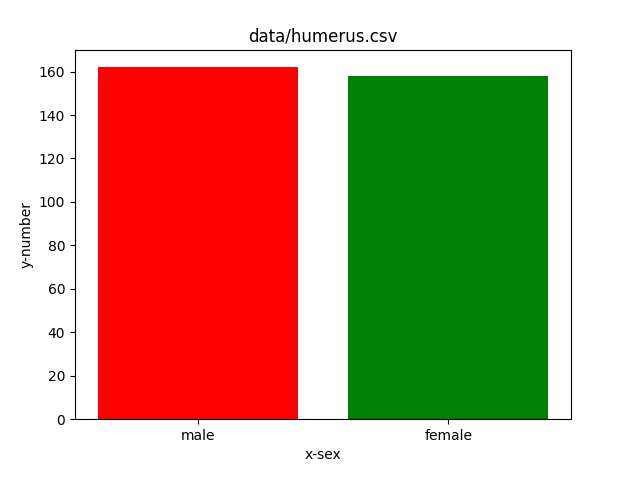
\includegraphics[height=8cm]{Imagini/plot_humerus_sex.png}}
\caption{Distributie dupa sex pentru humerus.}
\label{fig}
\end{figure}

\begin{figure}[h!]
\centerline{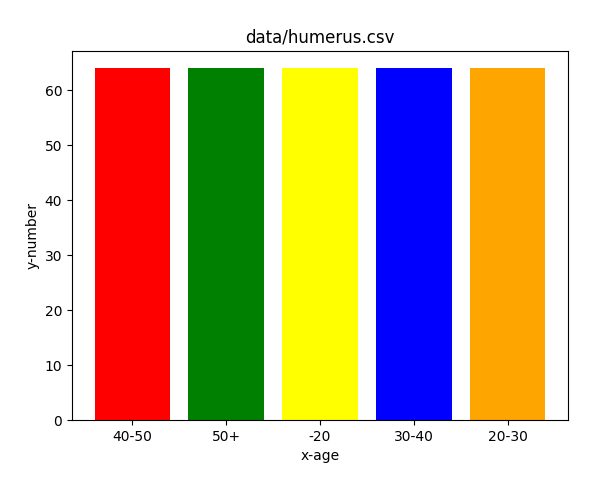
\includegraphics[height=10cm]{Imagini/plot_humerus_age.png}}
\caption{Distributie dupa varsta pentru humerus.}
\label{fig}
\end{figure}

\begin{figure}[h!]
\centerline{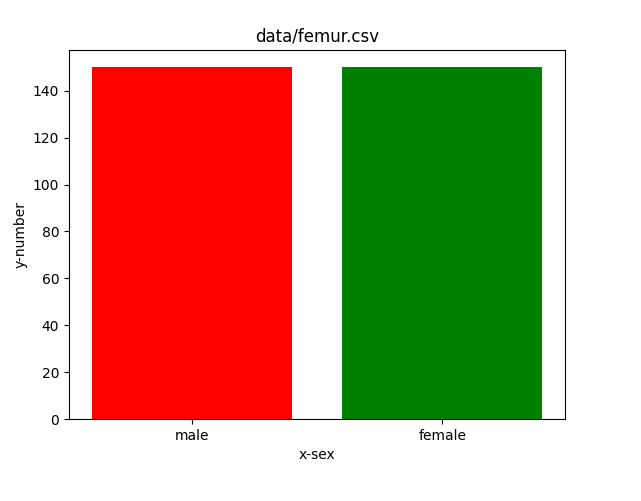
\includegraphics[height=10cm]{Imagini/plot_femur_sex.png}}
\caption{Distributie dupa sex pentru femur.}
\label{fig}
\end{figure}

\begin{figure}[h!]
\centerline{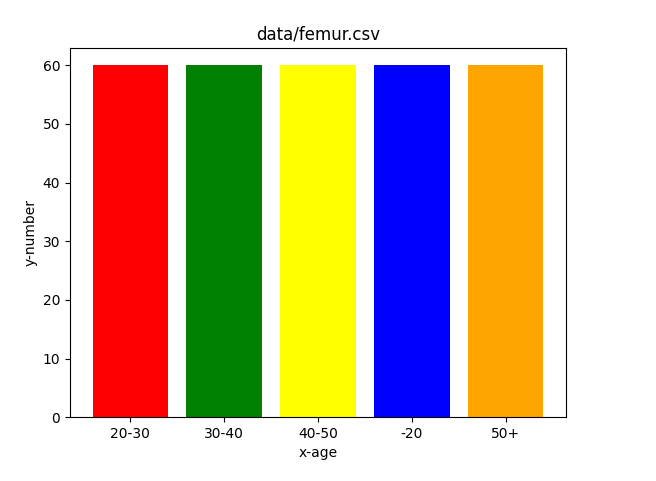
\includegraphics[height=10cm]{Imagini/plot_femur_age.png}}
\caption{Distributie dupa varsta pentru femur.}
\label{fig}
\end{figure}

\chapter{Problema stiintifica}
\label{section:problemaStiintifica}


\section{Definitia problemei}
\label{section:definitiaProblemei}
Subiectul abordat tine de domeniul istoriei si al arheologiei pentru a obtine informatii revelante despre obiectele identificate in santierele arheologice. Astfel se doreste o aplicatie care, plecand de la informatii deja studiate de arheologi umani, sa permita vizualizarea 3D a unor "descoperiri deja efectuate" in intregime sau partial, din diferite unghiuri, reliefand anumite detalii. Mai mult, ofera posibilitatea determinarii sexului sau varstei pe baza unor caracteristici numerice ale unui anumit tip de os. \newline \newline
Pentru simplitatea aplicatiei si usurinta folosirii exista o interfata grafica care va permite utilizatorului sa introduca caracteristicile pe baza carora se va stabili rezultatul. Dupa apasarea unui buton de trimitere a datelor, utilizatorul va fi intrebat daca este de acord ca datele introduse sa fie pastrate in baza de date pentru imbunatatirea solutiei. In urma procesarii datelor, utilizatorul va vedea care este sexul sau varsta osului specificat si va avea posibilitatea sa observe si in 3D cum ar arata acesta. \newline

\section{Algoritm machine learning - arbore de decizie}
\label{algoritmi}
Ca prim algoritm am folosit un arbore de decizie datorita simplitatii de a intelege cum mai exact se iau deciziile pentru a determina clasele din care face parte o instanta; este usor de inteles pentru o persoana din domeniul informaticii, dar si pentru orice alta persoana. \newline \newline
Pentru un arbore de decizie avem un nod radacina, noduri intermediare si noduri finale(frunze). Nodul radacina reprezinta atributul cel mai semnificativ, nodurile intermediare care reprezinta decizii de tip daca-atunci si frunzele care reprezinta clasa din care face parte o instanta. Pentru a determina rezultatul final practic se imparte setul de date in instante care respecta un anumit set de reguli. \newline \newline
Selectarea unui atribut ca fiind nod radacina se poate face folosind mai multi indici. Indexul Gini este varianta care se foloseste de clasa din Sklearn (DecisionTreeClassifier) daca nu este specificat alt index. Acesta este o metrica care masoara cat de des un element ales aleator este clasificat gresit; un index Gini mai mic inseamna un atribut care va fi preferat pentru a deveni nod radacina. In implementarea aplicatiei s-a folosit de asemenea un index Gini.

\section{Rezultate arbore de decizie}
\label{arboreDecizie}
O prima varianta de implementare pentru problema curenta de clasificare a folosit clasa din Sklearn (DecisionTreeClassifier) cu indexul Gini pentru a stabili nodul radacina. S-a folosit un set de date de dimensiune 100 care avea distirbutia descrisa ulterior. De asemenea, s-a creat un arbore in care se poate observa cum un nod intermediar reprezinta o decizie care se poate lua, ea fiind de tipul "daca conditia este adevarata, atunci mergi pe partea stanga a subarborelui, altfel pe partea dreapta; daca avem o frunza atunci ne oprim si returnam clasa corespunzatoare". \newline \newline
Folosind aceasta implementare am observat rezultate bune, avand o acuratete pentru determinarea sexului (probabilitatea ca un exemplu sa fie clasificat corect) de aproximativ 80\% cu un timp de executie redus pentru antrenarea arborelui. Totusi, un dezavantaj ce a fost remarcat a fost faptul ca arborele este destul de sensibil la modificarea datelor de intrare si o mica eroare de tipar poate da peste cap algoritmul(de exemplu, daca arborele primeste o instante care are numele caracteristicilor cu alt format fata de cum este dat in structura lui s-ar putea sa aiba probleme la asocierea valorilor cu sensul lor). \newline 
Initial acuratetea era de aproximativ 65\% atunci cand aveam setul de date initial cu peste 2000 de exemple, dar dupa ce am echilibrat setul de date si am ajuns aproximativ la celasi numar de femei si de barbati acuratetea a crescut la 80\%. \newline \newline
Am folosit pentru determinarea varstei tot un arbore de decizie, avand drept clase urmatoarele:
\begin{itemize}
  \item mai putin de 20 de ani
  \item intre 20 si 30 de ani
  \item intre 30 si 40 de ani
  \item intre 40 si 50 de ani
  \item peste 50 de ani
\end{itemize}
In acest caz am observat o acuratete destul de mica initial, in jur de 30\% si un arbore mult mai stufos si greu de parcurs. Timpul de executie nu se poate spune ca s-a marit sau nu, rezultatele se obtin destul de repede.Exact ca in cazul determinarii sexului, setul de date are aproximativ 1900 de exemple.\newline
Dupa echilibrarea setului de date s-a ajuns la o acuratete de aproximativ 45\%, ajungand la un numar mult mai redus de exemple cu care este antrenat algoritmul (aproximativ 300). \newline \newline

\section{Algoritm machine learning - retele neuronale}
\label{algoritmi}
Ca un al doilea algoritm am folosit o retea neuronala.
O retea neuronala este alcatuita din o multime de noduri (neuroni) dispuse ca un graf pe mai multe straturi (layere). Nodurile au rolul de a efectua calculi simple prin intermediul unei functii associate (functie de activare) si sunt conectate intre ei prin niste legaturi ponderate. Straturile sunt de 3 tipuri:  Strat de intrare care contine m neuroni unde m reprezinta numarul de caracteristici al unui obiect, Stratul de iesire care contine r neuroni,unde r reprezinta numarul de subclase si strat intermediar.

\section{Rezultate retele neuronale}
\label{rezultate}
Pentru rezolvarea problemei de clasificare a sexului am impartit datele ca fiind 80\% din ele date de antrenament si 20\% pentru date de testare. \newline
Reteaua neuronala este alcaturita din: 
\begin{itemize}
    \item stratul de intrare ce contine 4 neoroni
    \item strat intermediar de 20 de neoroni
    \item strat intermediar de 40 de neuroni
    \item stratul de iesire cu 2 neoroni
\end{itemize}

\noindent Pentru Humerus acuratetea modelului de clasificare de sex se afla intre 80-87\% in timp ce pentru femur acuratetea este intre 80-83\%. \newline

\noindent Pentru rezolvarea problemei de clasificare a varstei am impartit datele ca fiind 80\% din ele date de antrenament si 20\% pentru date de testare. Reteaua neuronala este alcatuita din:
\begin{itemize}
    \item stratul de intrare ce contine 4 neoroni
    \item strat intermediar de 20 de neoroni
    \item strat intermediar de 10 de neuroni
    \item stratul de iesire cu 5 neoroni
\end{itemize}

\noindent Pentru Humerus acuratetea modelului de clasificare de varsta se afla intre 18-27\% in timp ce pentru femur acuratetea este intre 19-27\%. \newline 
 
\begin{figure}[h!]
\centerline{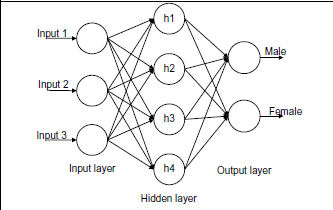
\includegraphics{Imagini/retea.PNG}}
\caption{Structura retelei neuronale pentru clasificarea in functie de sex.}
\label{fig}
\end{figure}

\begin{figure}[h!]
\centerline{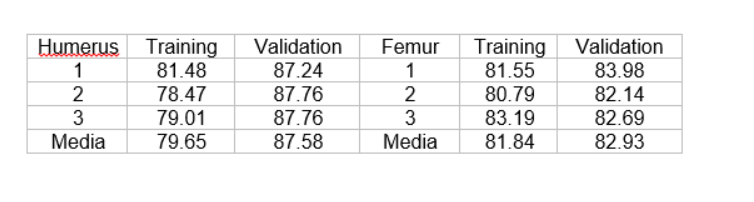
\includegraphics[height=8cm,width=20cm]{Imagini/tabel_date_acuratete.PNG}}
\caption{Rezultate obtinute pentru mai multe testari pentru sex.}
\label{fig}
\end{figure}

\begin{figure}[h!]
\centerline{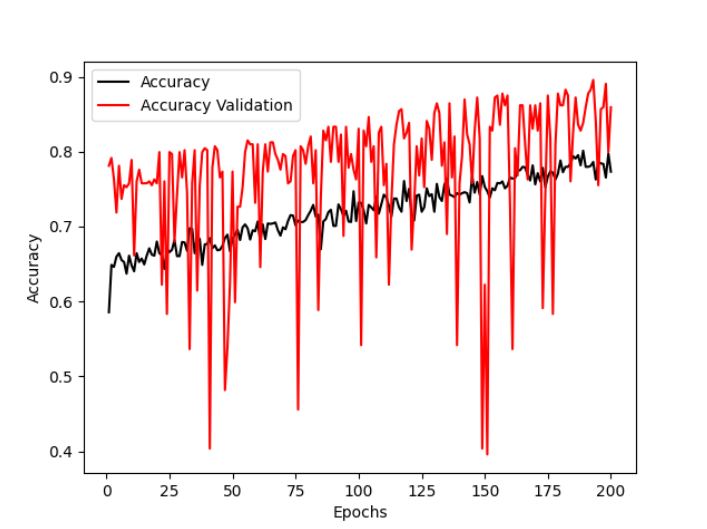
\includegraphics[height=10cm]{Imagini/acuratete_humerus.png}}
\caption{Acuratetea obtinuta pentru humerus in functie de numarul de epoci pentru sex.}
\label{fig}
\end{figure}

\begin{figure}[h!]
\centerline{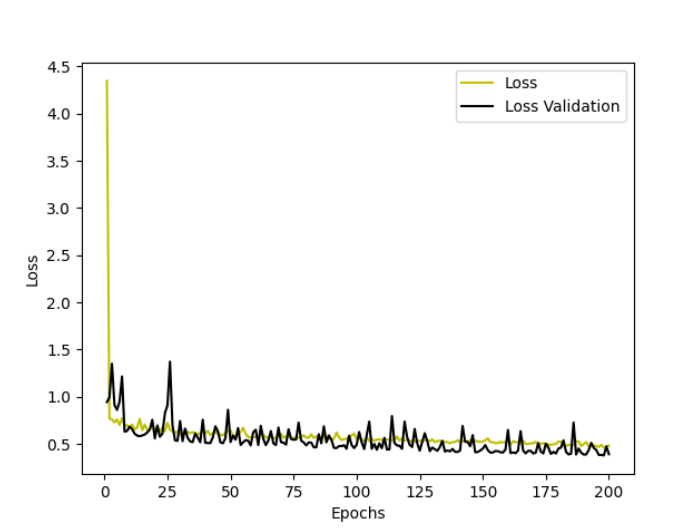
\includegraphics[height=10cm]{Imagini/loss_humerus.png}}
\caption{Loss obtinut pentru humerus in functie de numarul de epoci pentru sex.}
\label{fig}
\end{figure}

\begin{figure}[h!]
\centerline{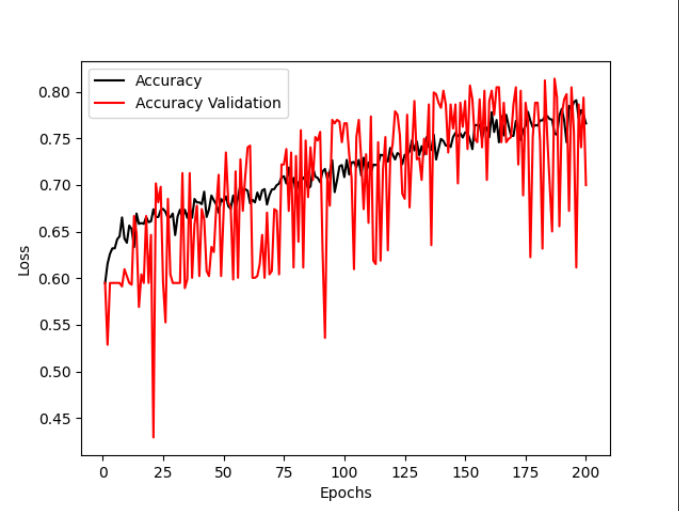
\includegraphics[height=10cm]{Imagini/acuratete_femur.png}}
\caption{Acuratetea obtinuta pentru femur in functie de numarul de epoci pentru sex.}
\label{fig}
\end{figure}

\begin{figure}[h!]
\centerline{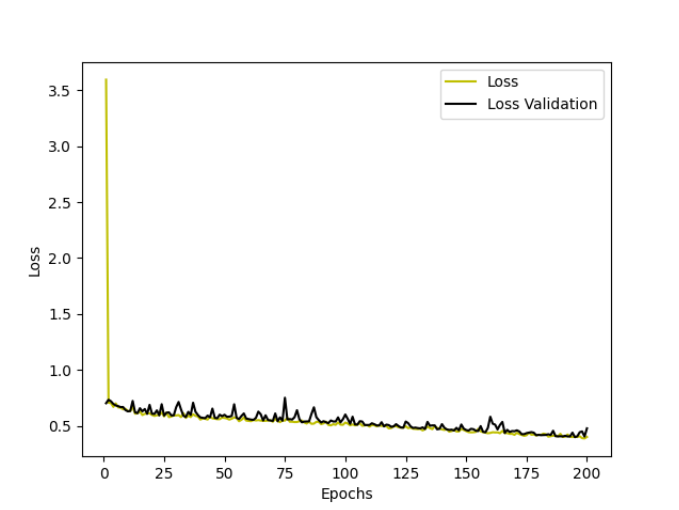
\includegraphics[height=10cm]{Imagini/loss_femur.png}}
\caption{Loss obtinut pentru femur in functie de numarul de epoci pentru sex.}
\label{fig}
\end{figure}

\begin{figure}[h!]
\centerline{
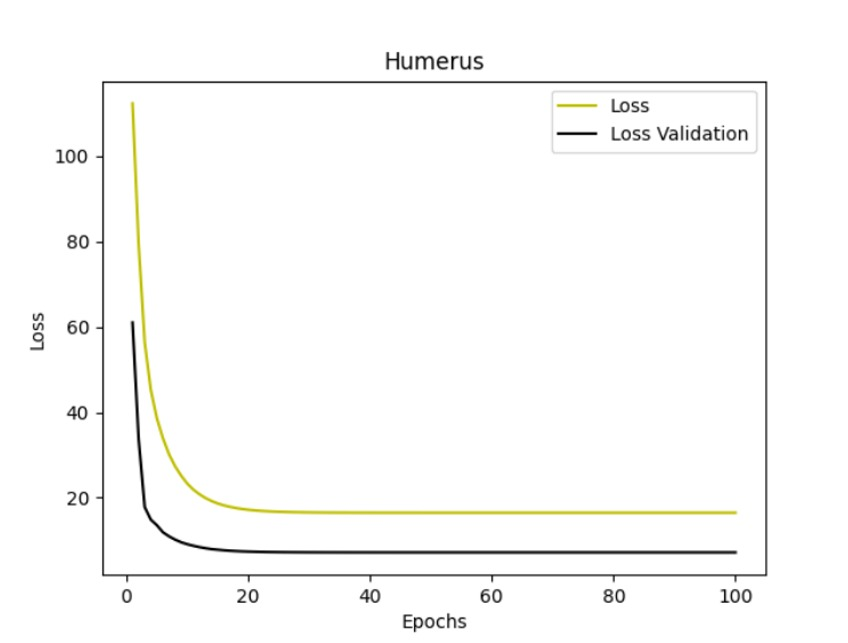
\includegraphics[height=10cm]{Imagini/humerus_loss_age.png}}
\caption{Loss obtinut pentru humerus in functie de numarul de epoci pentru varsta.}
\label{fig}
\end{figure}

\begin{figure}[h!]
\centerline{
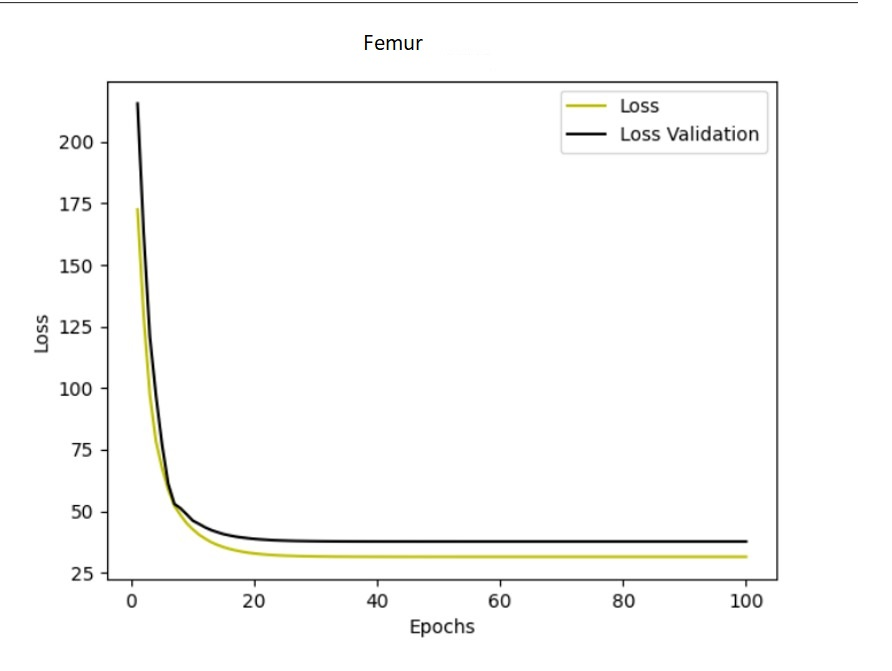
\includegraphics[height=10cm]{Imagini/femur_loss_age.png}}
\caption{Loss obtinut pentru femur in functie de numarul de epoci pentru varsta.}
\label{fig}
\end{figure}

\begin{figure}[h!]
\centerline{
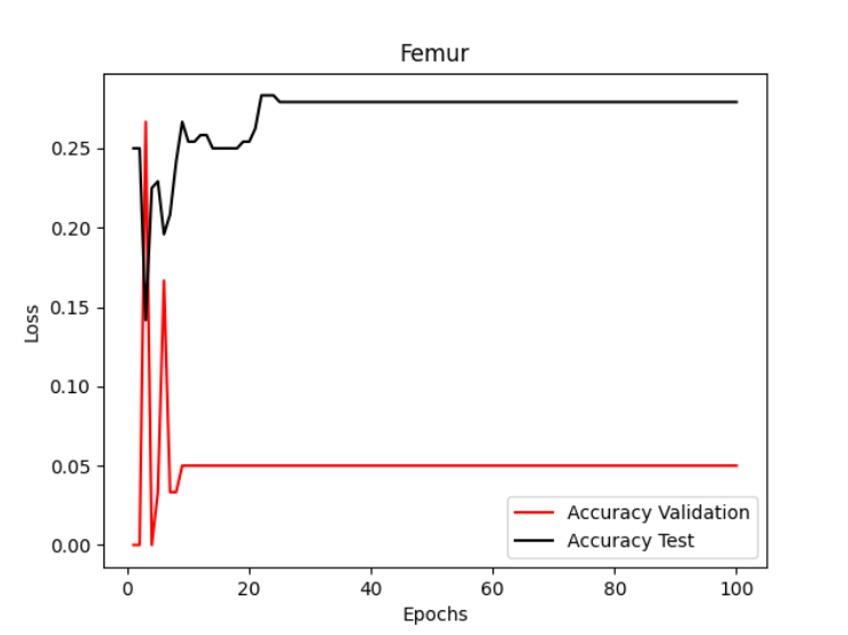
\includegraphics[height=10cm]{Imagini/femur_acc_age.png}}
\caption{Acuratete obtinuta pentru femur in functie de numarul de epoci pentru varsta.}
\label{fig}
\end{figure}

\begin{figure}[h!]
\centerline{
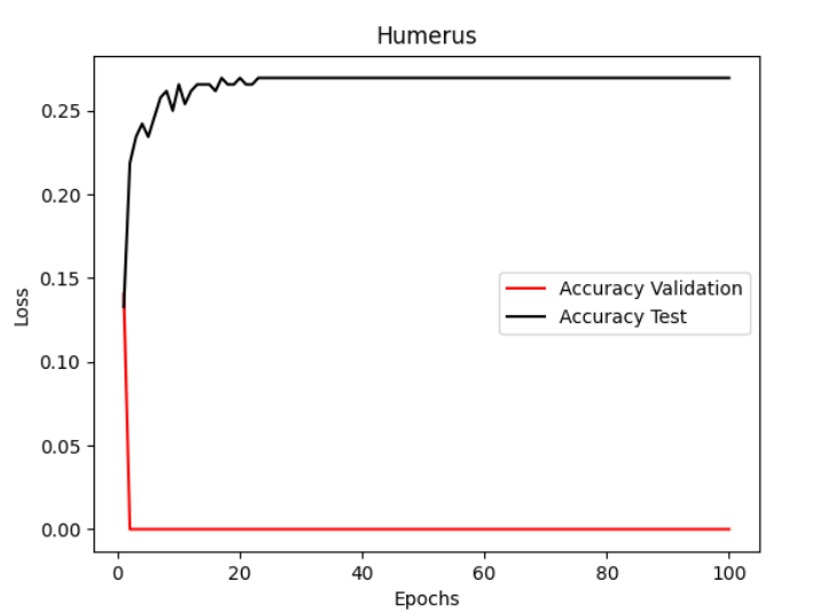
\includegraphics[height=10cm]{Imagini/humerus_acc_age.png}}
\caption{Acuratete obtinuta pentru humerus in functie de numarul de epoci pentru varsta.}
\label{fig}
\end{figure}

\begin{figure}
\centerline{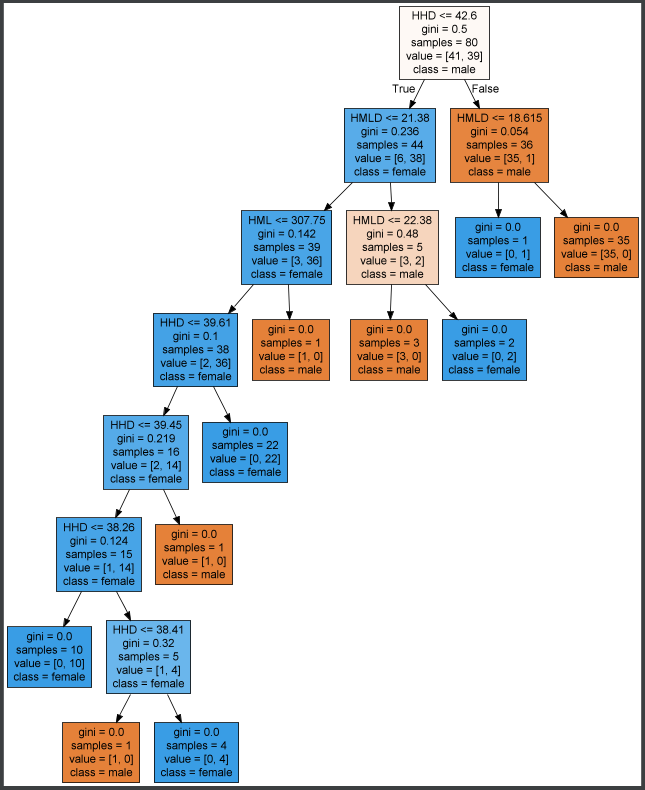
\includegraphics{Imagini/tree_sex_humerus_100.PNG}}
\caption{Arbore generat pentru un set de date cu 100 de exemple, clasificare sex pentru humerus.}
\label{fig}
\end{figure}

\begin{figure}
\centerline{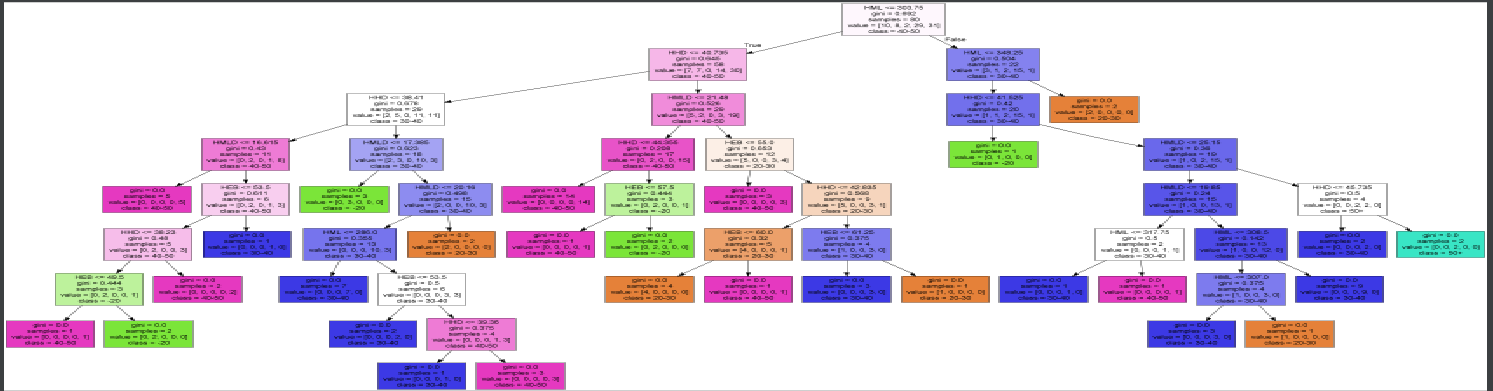
\includegraphics[width=20cm,keepaspectratio]{Imagini/tree_age_humerus_100.png}}
\caption{Arbore generat pentru un set de date cu 100 de exemple, clasificare varsta pentru humerus.}
\label{fig}
\end{figure}

\begin{figure}
\centerline{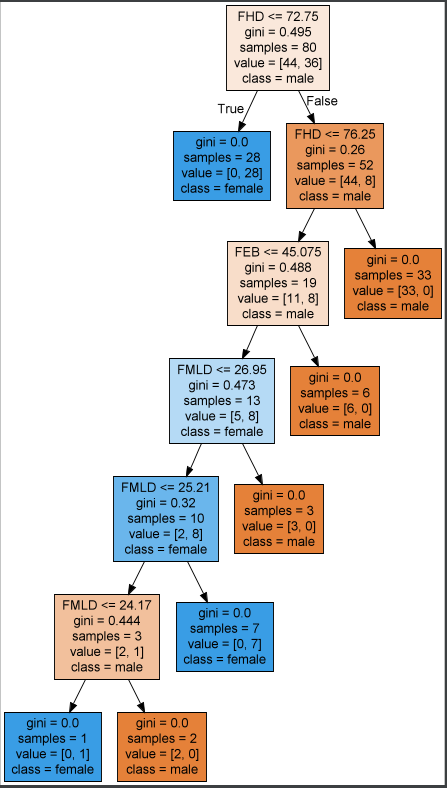
\includegraphics{Imagini/tree_sex_femur_100.PNG}}
\caption{Arbore generat pentru un set de date cu 100 de exemple, clasificare sex pentru femur.}
\label{fig}
\end{figure}

\begin{figure}
\centerline{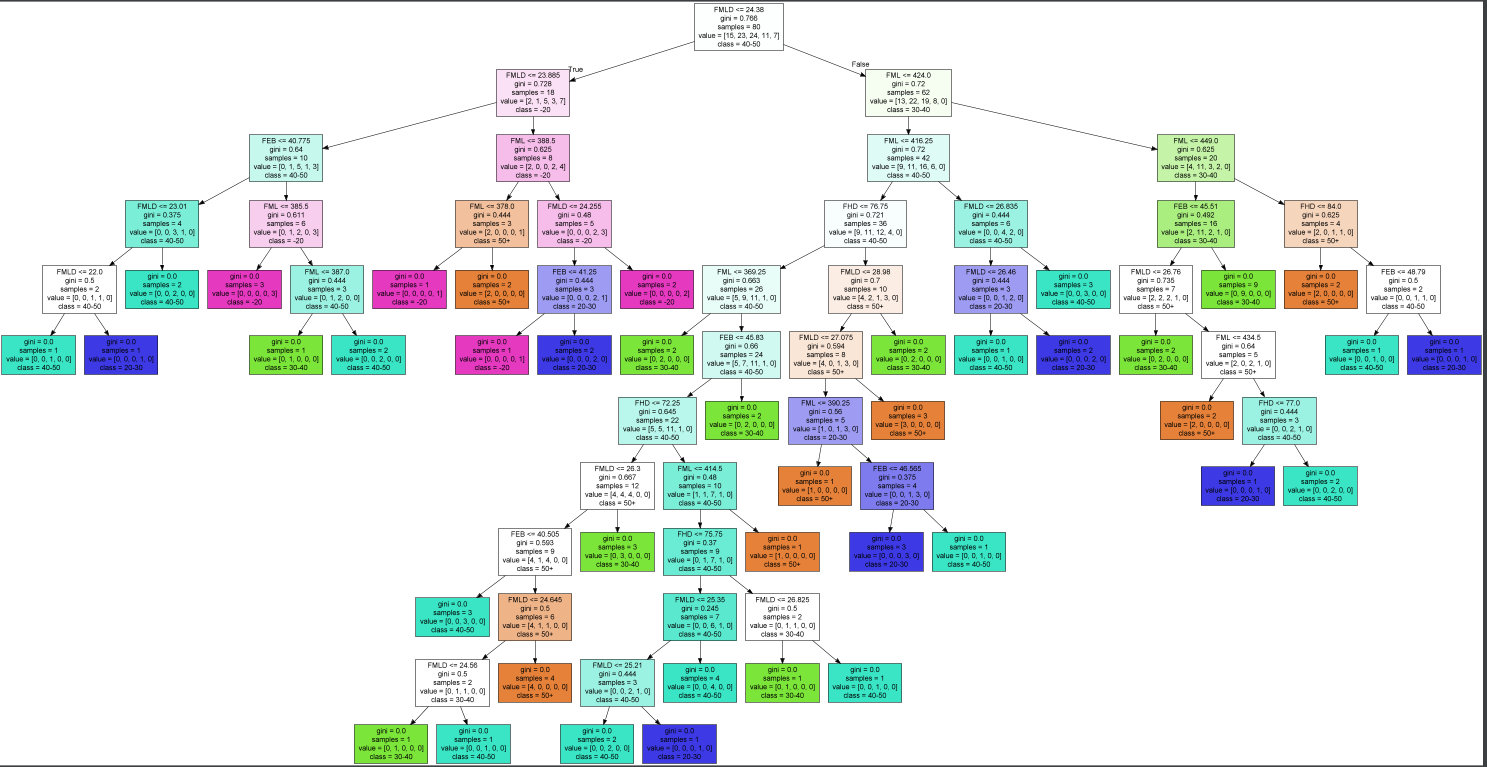
\includegraphics[width=20cm,keepaspectratio]{Imagini/tree_age_femur_100.png}}
\caption{Arbore generat pentru un set de date cu 100 de exemple, clasificare varsta pentru femur.}
\label{fig}
\end{figure}

\chapter{SOTA (State Of The Art)}
\label{chapter:sota}

\section{Arbore de decizie}
\label{sotaArboreDecizie}
Lucrarea stiintifica care a stat la baza alegerii de a folosi arbori de decizie pentru a determina varsta a fost \textit{SEX IDENTIFICATION IN ARCHAEOLOGICAL REMAINS USING DECISION TREE LEARNING}, avandu-i ca autori pe Ioan-Gabriel Mircea, Gabriela Czibula si Mara-Renata Petrusel, an 2015. \newline \newline
S-a folosit algoritimul ID3 (Iterative Dichotomiser 3) care foloseste un set de date S pe care il considera nod radacina. La fiecare iteratie a algoritmului se itereaza prin fiecare atribut nefolosit din S si se calculeaza entropia acelui atribut. Se selecteaza atributul cu cea mai mica entropie si astfel se imparte setul de date in mai multe subseturi. Algortimul se poate opri in unul din cazurile:
\begin{itemize}
  \item fiecare element din subset apartine aceleasi clase, caz in care nodul este transformat in frunza si etichetat cu clasa exemplelor din subset
  \item nu mai exista atribute ce pot fi selectate si exemplele nu fac parte din aceeasi clasa; in acest caz nodul este transformat in frunza si este etichetat cu clasa cea mai comuna din exemplele subsetului
  \item nu mai exista exemple in subset care se intampla in momentul in care niciun exemplu din setul initial nu a fost gasit sa i se potriveasca o valoare cu atributul selectat; in acest caz se creeaza un nod frunza care este etichetat cu clasa cea mai comuna a exemplelor din setul initial
\end{itemize}

\hfill \break
\hfill \break
Setul de date cu care s-a lucrat a continut 200 de barbati si 200 de femei. In primul caz de testare un os a fost caracterizat de 10 masuratori legate de radius, in al doilea caz au fost 9 caracteristici ce tineau de antebrat, iar al treilea caz a fost reuniunea datelor din primele doua cazuri, deci s-a ajuns la 19 caracteristici pentru antrebrat si radius. \newline  \newline
Acuratetea cea mai buna obtinuta a fost de 86\% pentru primul caz, pentru al doilea a fost 87\% si pentru al treilea s-a reusit o acuratete de 88\%. \newline \newline
Astfel, comparand cu rezultatele obtinute cu aborele de decizie folosit in aceasta aplicatie se poate observa ca diferenta nu este atat de mare si acuratetea se apropie de ceea ce s-a obtinut in articolul stiintific. Una din diferente este faptul ca s-au folosit 200 de barbati si 200 de femei in lucrare, iar in aplicatia curenta s-au folosit aproximativ 1000 de barbati si aproximativ 1000 de femei. A doua diferenta consta in numarul de caracteristici ce s-au folosit pentru antrenarea algoritmului. In cazul aplicatiei curente s-au folosit 4 masuratori ale unui humerus ( HML - humerus maximum length,HEB - humerus epicondylar breadth, HHD - humer head diameter, HMLD - humerus 50\% diaphyseal mediolateral diameter). \newline \newline

\section{Retele neuronale}
\label{sotaReteleNeuronale}
Lucrare stiintifica care sta la baza alegerii de a folosi un ANN pentru a determina sexul este \textit{Determination of Gender from Pelvic Bones and Patella in Forensic Anthropology:
A Comparison of Classification Techniquees}. 

\hfill \break

\noindent In acesta lucrare s-a folosit un algoritm de Back propagation Neural Network (BPNN) iar identificarea sexului unei prsoane se face pe baza oaselor perviene. Pentru antrenarea modelului s-au folosit 136 de oase pelviene (55 feminine si 81 masculine), unde 70\% din ele au fost folosite pentru antrenarea modelului si 30\% pentru testare. Modelul a fost antrenat pe baza inailtime, latimii si grosimii osului pelvian. 

\hfill \break
\hfill \break

\noindent Acuratetea optinuta pentru osul pelvian drept este de 98.5\% (datele de antrenament) si 98.3\% (datele de testare) iar pentru osul pervian stang este de 98.49\% (datele de testare) si 86.6\% (datele de antrenament).

\hfill \break

\noindent Asadar comparative cu rezultatele optinute la modelul implementat de noi care are o acuratete de 79.65\%(datele de training), 87.58\%(datele de testare) pentru humerus si 81.84(date de training), 82.93 (date de testare)
pentru femur, modelul din lucrarea stiintifica prezentata da rezultate mult mai bune.

\chapter{Imbunatatirea aplicatiei}
\label{chapter:complexitate}

\section{Arbori de decizie}
\label{arboriDeDecizieComplecitate}
Comparand aplicatia cu varianta initiala se poate observa o imbunatatire a acuratetei, dar si a timpului de executie. Prelucrand setul de date a fost redus numarul de instante cu care se antreneaza algoritmul (pentru femur exista 300, iar pentru humerus 320) astfel incat datele sa fie distribuite egal din punctul de vedere al sexului, dar si al varstei. Cu aceasta modificare acuratetea pentru sex a crescut de la aproximativ 65\% la aproximativ 85\%, iar pentru varsta acuratetea a crescut de la aproximativ 30\% la aproximativ 45\%. De asemenea, reducerea numarului de instante cu care se lucreaza de la aproximativ 2000 la aproximativ 300 a imbuntatit si timpul de executie, determinarea sexului si varstei fiind mult mai rapide.Astfel, masurand timpul de executie avem 0.103 secunde pentru determinarea sexului si 0.000998 secunde pentru determinarea varstei fata de cel putin 1-2 secunde cat era initial (pentru aceste rezultate s-a folosit libraria time din Python, iar timpul a fost masurat ca diferenta intre momentul in care incepe antrenarea arborelui de decizie si momentul in care s-a terminat antrenarea si s-a prezis valoarea pentru instanta data).

\section{Retele neuronale}
\label{reteleComplexitate}
Comparand aplicatia cu varianta initiala se poate observa o imbunatatire a acuratetei. Prelucrand setul de date, a fost redus numarul de instante cu care se antreneaza algoritmul (pentru femur exista 300, iar pentru humerus 320) astfel incat datele sa fie distribuite egal din punctul de vedere al sexului, am modificat learning rate-ul astfel incat acesta sa scada pe parcurs ce modelul se antreneaza si a crescut numarul de epoci de la 200 la 800.
Cu aceste modificari acuratetea pentru detectare de sex a crescut de la 79.65\%(datele de training), 87.58\%(datele de testare) la 88,6\%(datele de training), 96,8\%(datele de testare) pentru humerus si de la 81.84\%(date de training), 82.93\% (date de testare) la 90.83\%(date de training), 93.33\% (date de testare) pentru femur. \newline \newline

\section{Tehnici de evaluare}
\label{tehnici}
Functia de loss este functia care calculeaza distanta dintre iesirea curenta a algoritmului si iesirea asteptata. Este o metoda de a evalua modul in care algoritmul modeleaza datele. (vezi figura \ref{loss_femur} si \ref{loss_humerus})
\newline

\noindent O matrice de confuzie este un rezumat al rezultatelor predictiei pentru o problema de clasificare. Numarul de predictii corecte si incorecte este rezumat cu valori de numarare si impartit pe fiecare clasa. Aceasta este cheia matricei de confuzie. Matricea de confuzie arata modalitatile in care modelul de clasificare este confuz cand face predictii. (vezi \ref{matrice_confuzie_sex}, \ref{matrice_confuzie_varsta}, \ref{matrice_confuzie_femur_sex_retea}, \ref{matrice_confuzie_sex_humeru_retea})

\hfill \break
\hfill \break
\hfill \break

\begin{figure}
  \centering
  \begin{minipage}[b]{0.4\textwidth}
    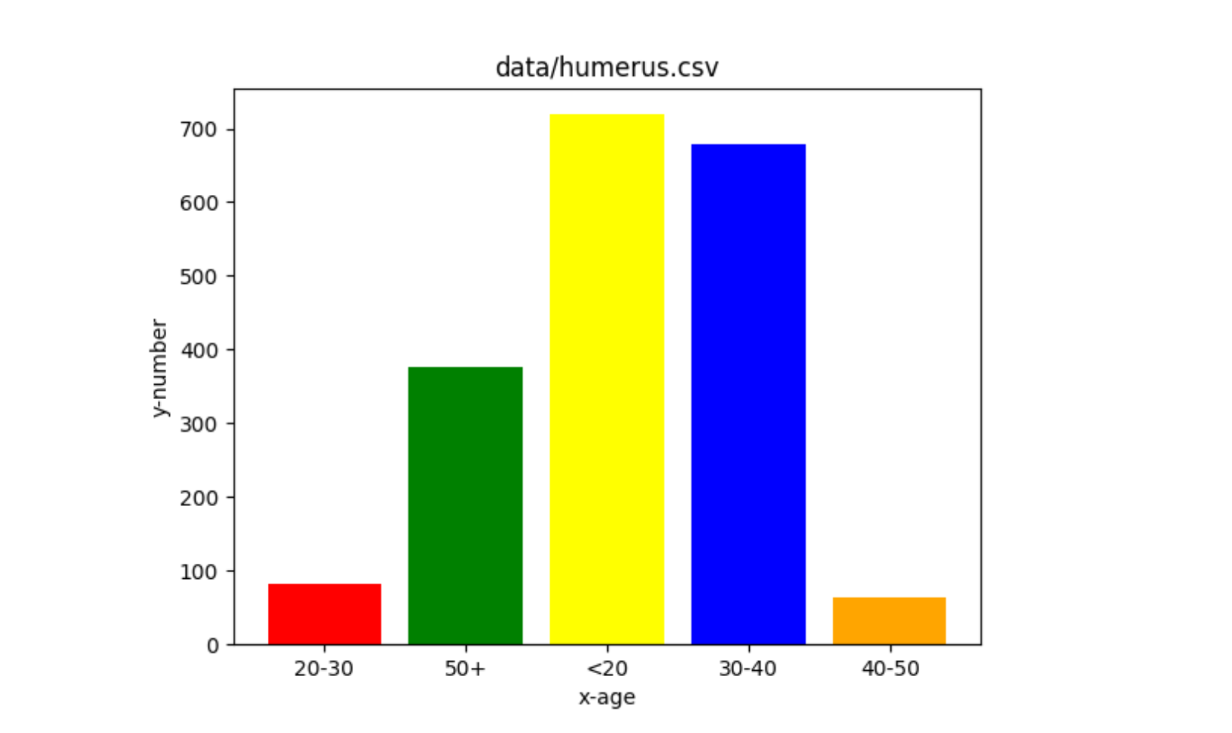
\includegraphics[width=10cm]{Imagini/plot_age_init.PNG}
    \caption{Distributie varsta initiala.}
  \end{minipage}
  \hfill
  \begin{minipage}[b]{0.4\textwidth}
    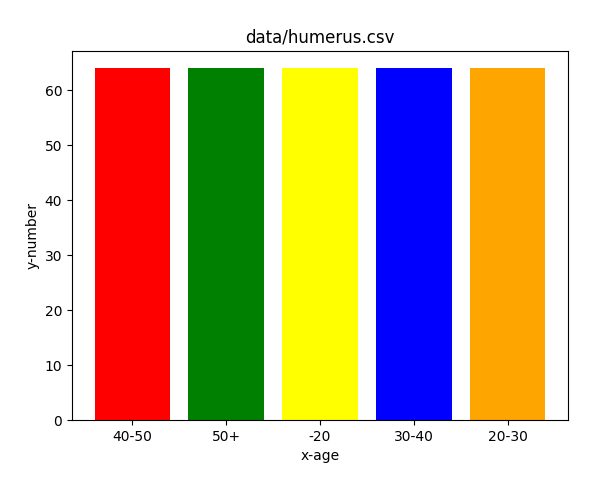
\includegraphics[width=9cm,height=10cm]{Imagini/plot_humerus_age.png}
    \caption{Distributie varsta actuala.}
  \end{minipage}
\end{figure}

\begin{figure}[!h]
  \centering
  \begin{minipage}[b]{0.4\textwidth}
    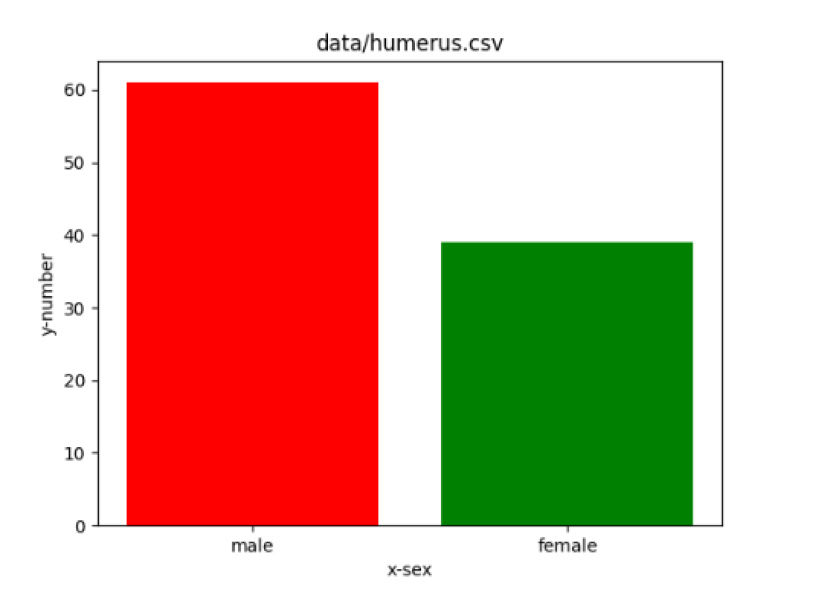
\includegraphics[width=10cm,height=10cm]{Imagini/plot_init_sex.PNG}
    \caption{Distributie sex initiala.}
  \end{minipage}
  \hfill
  \begin{minipage}[b]{0.4\textwidth}
    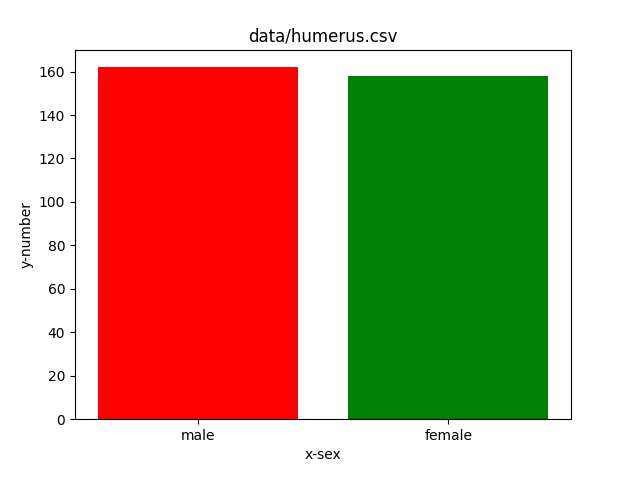
\includegraphics[width=9cm]{Imagini/plot_humerus_sex.png}
    \caption{Distributie sex actuala.}
  \end{minipage}
\end{figure}

\begin{figure}
    \centering
    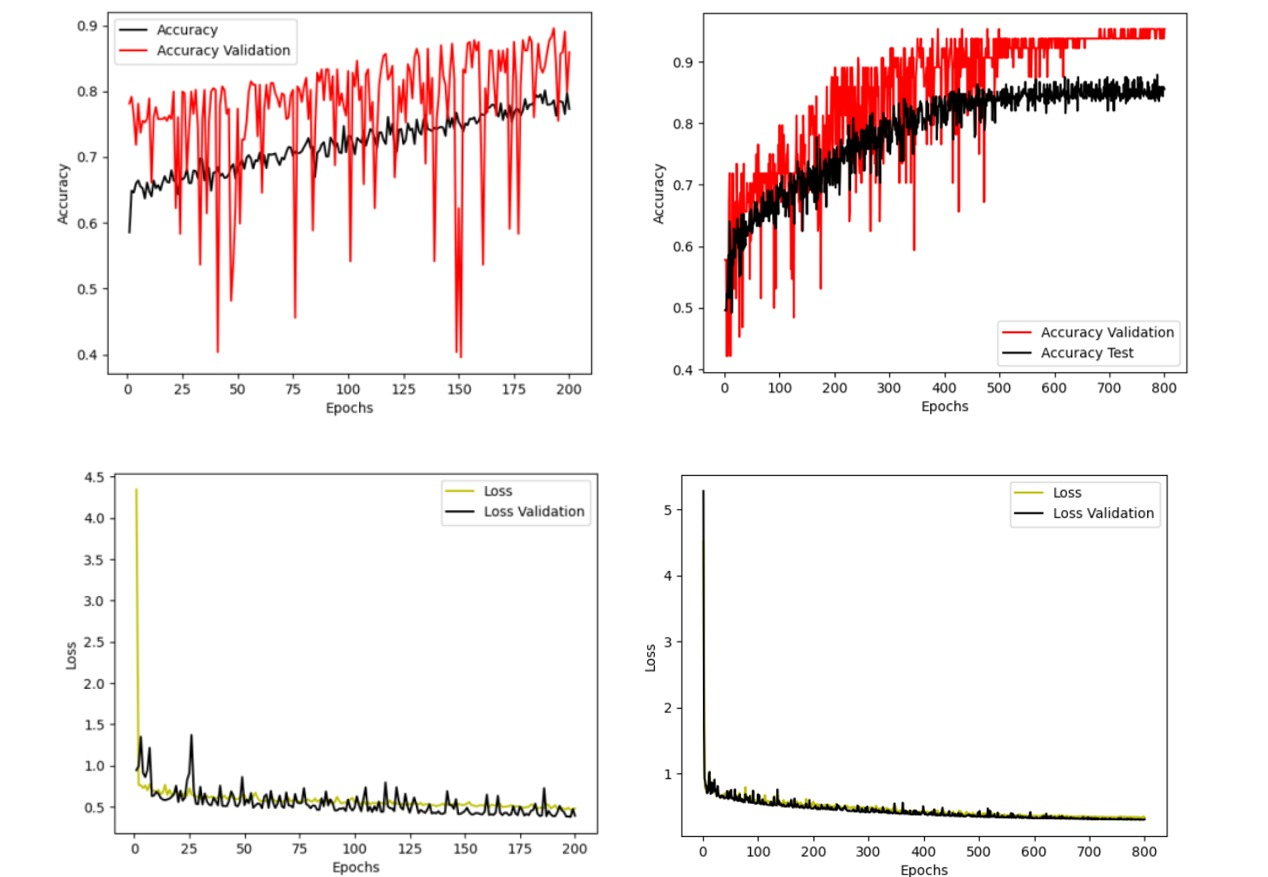
\includegraphics[width=20cm,height=15cm]{Imagini/loss_acuratete_femur.png}
    \caption{Acuratetea si loss-ul initial si actual pentru femur.}
    \label{loss_femur}
\end{figure}

\begin{figure}
    \centering
    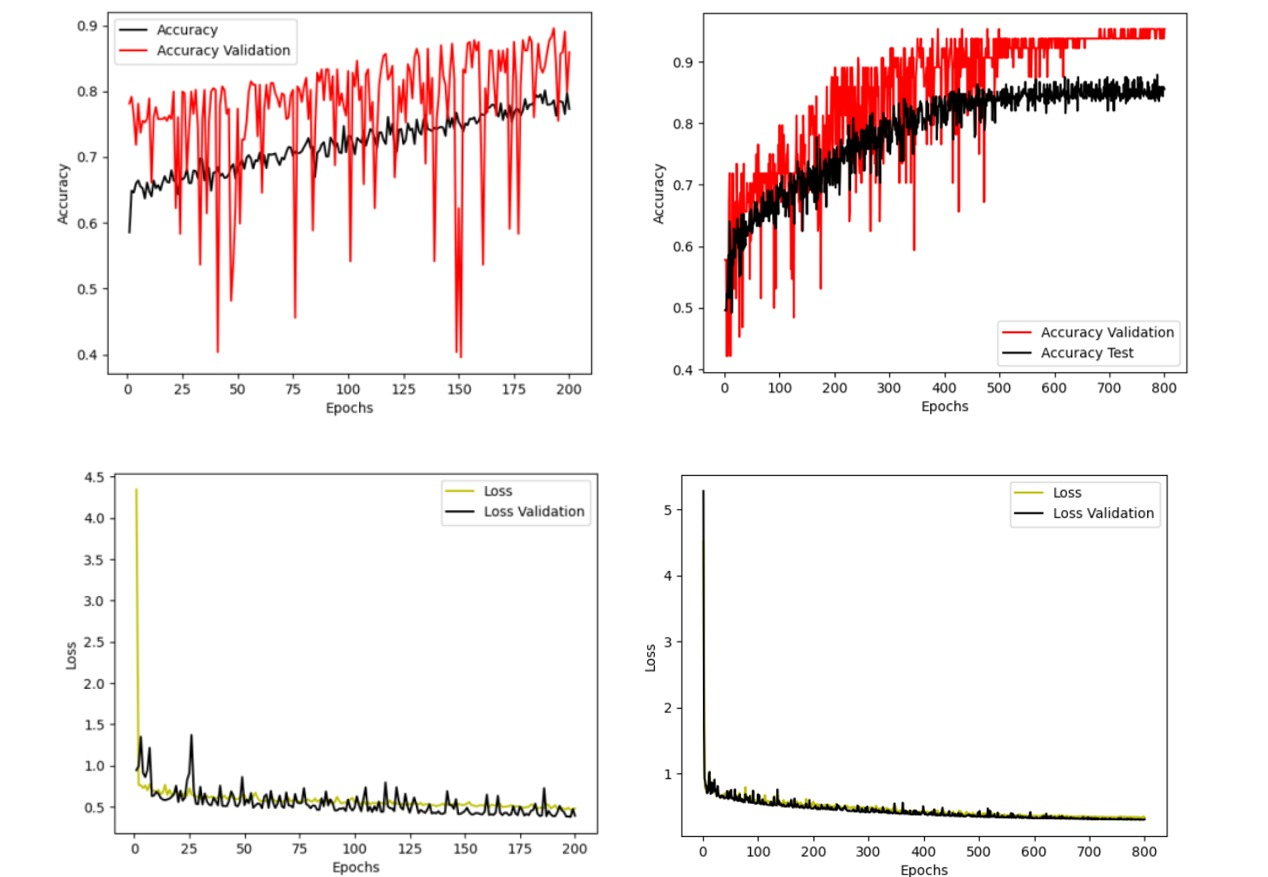
\includegraphics[width=20cm,height=15cm]{Imagini/loss_acuratete_humerus.png}
    \caption{Acuratetea si loss-ul initial si actual pentru humerus.}
    \label{loss_humerus}
\end{figure}

\begin{figure}
    \centering
    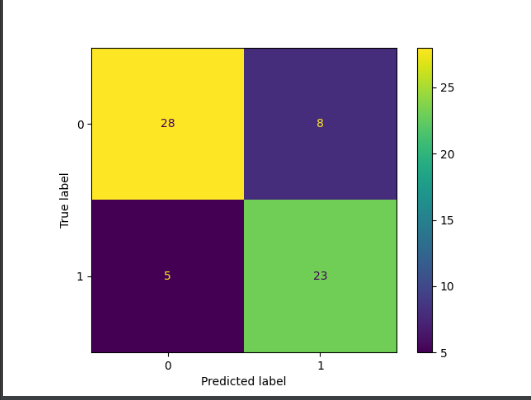
\includegraphics[height=10cm]{Imagini/matrice_confuzie_sex_arbore.PNG}
    \caption{Matricea de confuzie sex humerus(arbore de decizie).}
    \label{matrice_confuzie_sex}
\end{figure}

\begin{figure}
    \centering
    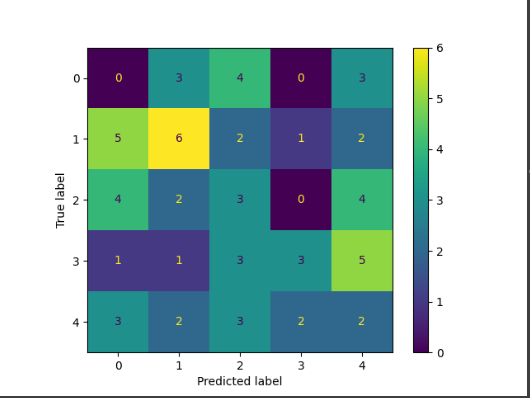
\includegraphics[height=10cm]{Imagini/matrice_confuzie_varsta_arbore_decizie.png}
    \caption{Matricea de confuzie varsta humerus(arbore de decizie).}
    \label{matrice_confuzie_varsta}
\end{figure}

\begin{figure}
    \centering
    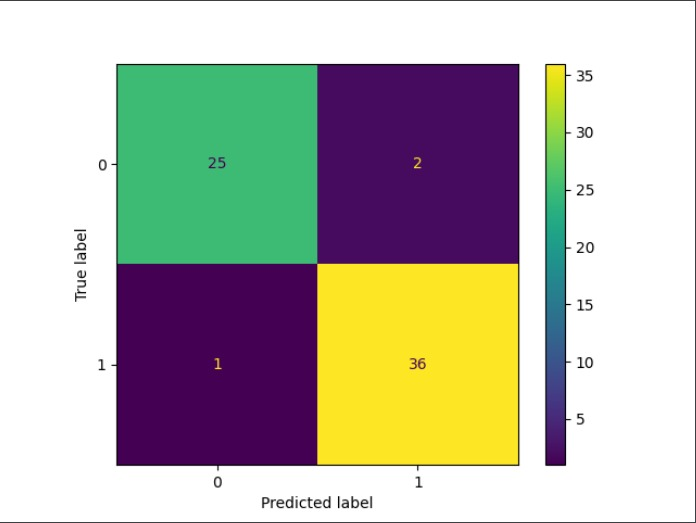
\includegraphics[height=10cm]{Imagini/matrice_confuzie_sex_retea.png}
    \caption{Matricea de confuzie sex humerus(retea neuronala).}
    \label{matrice_confuzie_sex_humerus_retea}
\end{figure}

\begin{figure}
    \centering
    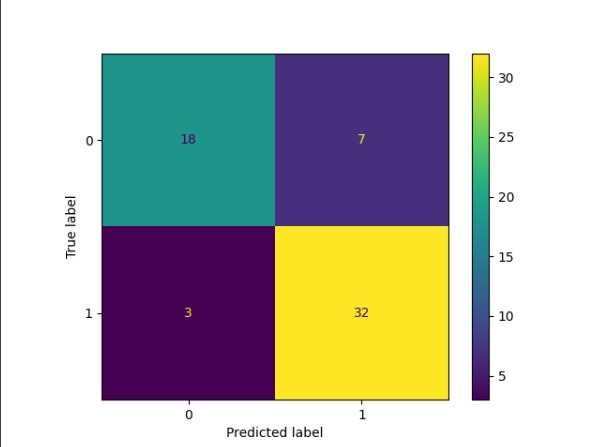
\includegraphics[height=10cm]{Imagini/matrice_confuzie_sex_femur_retea.png}
    \caption{Matricea de confuzie sex femur(retea neuronala).}
    \label{matrice_confuzie_femur_sex_retea}
\end{figure}

\chapter{Analiza statistica a algoritmilor}
\label{anaizaStatistica}
S-a realizat o analiza pe diferite seturi de date atat pentru humerus, cat si pentru femur urmarind acuratetea rezultata pentru determinarea sexului, dar si pentru determinarea varstei. Astfel, pentru fiecare tip de os s-au folosit cinci seturi de date cu diferite procente folosite la extragerea datelor de test din tot setul de date. Astfel, s-au folosit urmatoarele valori pentru a imparti datele: 20\%, 40\%, 80\%, 35\% si 70\%.

\section{Arbori de decizie (vezi \ref{plot_arbori})} 
\label{analizaArboriSex}
Determinare sex pentru humerus
\begin{itemize}
    \item media acuratetilor este: 81.41
    \item interval de incredere: [78.12, 84.37]
\end{itemize}

\noindent Determinare varsta pentru humerus
\begin{itemize}
    \item media acuratetilor este: 28.73
    \item interval de incredere: [20.31, 33.59]
\end{itemize}

\noindent Determinare sex pentru femur
\begin{itemize}
    \item media acuratetilor este: 87.08
    \item interval de incredere: [84.76, 88.75]
\end{itemize}

\noindent Determinare varsta pentru femur
\begin{itemize}
    \item media acuratetilor este: 29.59
    \item interval de incredere: [23.33, 41.66]
\end{itemize}

\begin{figure}[!h]
    \centering
    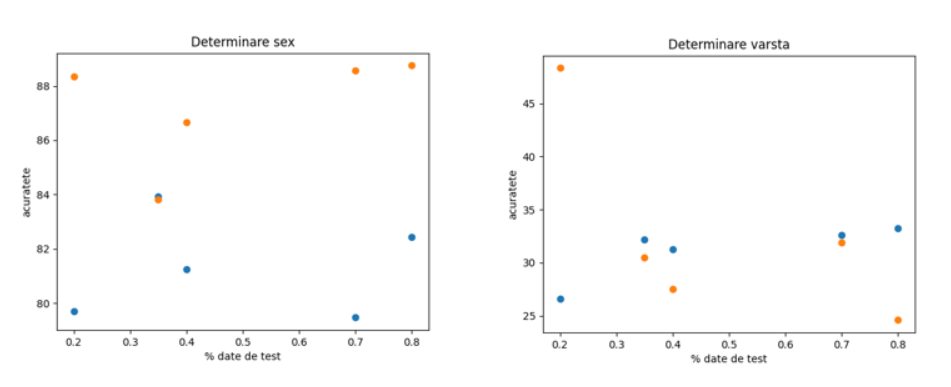
\includegraphics[width=18cm]{Imagini/plot_acc_arbori.PNG}
    \caption{Reprezentare grafica a relatiei dintre acuratete si dimensiunea setului de date.\newline (albastru - humerus, portocaliu - femur)}
    \label{plot_arbori}
\end{figure}

\section{Retele neuronale (vezi \ref{plot_retele})}
\label{analizaReteleSex}

\noindent Determinare sex pentru humerus
\begin{itemize}
    \item media acuratetilor este: 82.48
    \item interval de incredere: [71.59, 96.875]
\end{itemize}

\noindent Determinare varsta pentru humerus
\begin{itemize}
    \item media acuratetilor este: 25.59
    \item interval de incredere: [14.73, 53.125]
\end{itemize}

\noindent Determinare sex pentru femur
\begin{itemize}
    \item media acuratetilor este: 85.13
    \item interval de incredere: [80.47, 90.0]
\end{itemize}

\noindent Determinare varsta pentru femur
\begin{itemize}
    \item media acuratetilor este: 27.56
    \item interval de incredere: [0.83, 60.00]
\end{itemize}

\begin{figure}[!h]
    \centering
    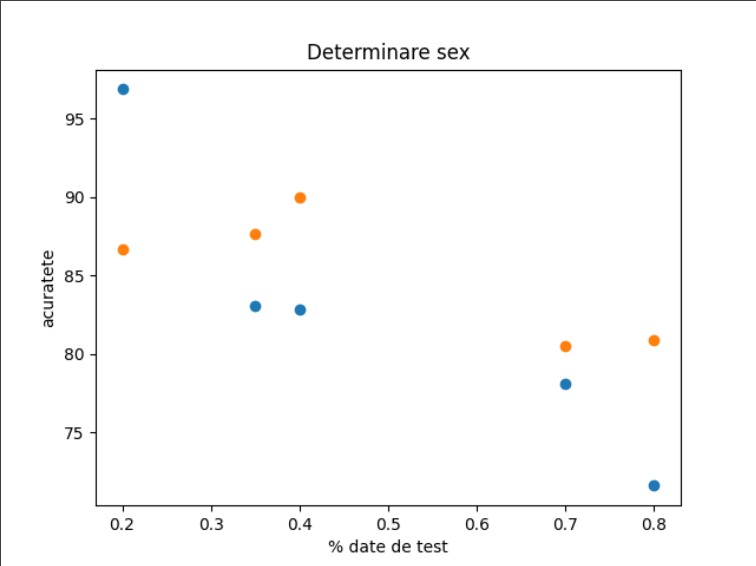
\includegraphics[width=18cm,height=8cm]{Imagini/plot_acurateti_retea_sex.png}
    \caption{Reprezentare grafica a relatiei dintre acuratete si dimensiunea setului de date pentru reteaua neuronala.(albastru - humerus, portocaliu - femur)}
    \label{plot_retele}
\end{figure}

\section{Rezultatele analizei pentru determinarea sexului (vezi \ref{plot_sex})}
\label{analizaRezultate}

\noindent Folosind arbori de decizie am obtinut un interval de incredere de [78.12, 84.37] pentru humerus, in timp ce folosind reteaua neuronala am obtinut [71.59, 96.875]. Cele doua intervale obtinute nu sunt disjuncte, deci nu se poate exprima care algoritm este mai eficient pentru setul de date de la humerus. 
\newline

\noindent Folosind arbori de decizie am obtinut un interval de incredere de [84.76, 88.75] pentru femur, in timp ce folosind reteaua neuronala am obtinut [80.47, 90.0]. Analog ca pentru humerus, cele doua intervale nu sunt disjuncte, deci nu se poate afirma care algoritm este mai eficient pe acest set de date.
\newline

\noindent Concluzionand, pentru determinarea sexului, atat pentru humerus, cat si pentru femur, cei doi algoritmi de machine learning propusi dau rezultate similare, neputand afirma ca unul este mai bun ca celalalt.

\section{Rezultatele analizei pentru determinarea varstei (vezi \ref{plot_age})}
\label{analizaRezultate}

\noindent Folosind arbori de decizie am obtinut un interval de incredere de [20.31, 33.59] pentru humerus, in timp ce folosind reteaua neuronala am obtinut [14.73, 53.125]. Cele doua intervale obtinute nu sunt disjuncte, deci nu se poate exprima care algoritm este mai eficient pentru setul de date de la humerus. 
\newline \newline \newline

\noindent Folosind arbori de decizie am obtinut un interval de incredere de [23.33, 41.66] pentru femur, in timp ce folosind reteaua neuronala am obtinut [0.83, 60.00]. Analog ca pentru humerus, cele doua intervale nu sunt disjuncte, deci nu se poate afirma care algoritm este mai eficient pe acest set de date.
\newline

\noindent Concluzionand, pentru determinarea varstei, atat pentru humerus, cat si pentru femur, cei doi algoritmi de machine learning propusi dau rezultate similare, neputand afirma ca unul este mai bun ca celalalt. \newline

\begin{figure}[!h]
    \centering
    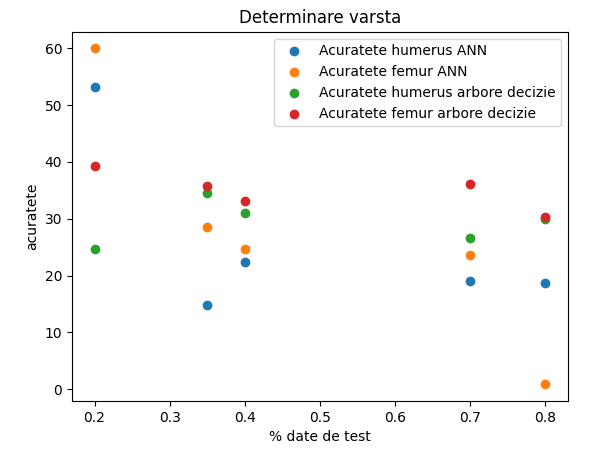
\includegraphics[width=18cm, height=10cm]{Imagini/plot_age.PNG}
    \caption{Reprezentare grafica a celor doi algoritmi pentru determinarea sexului.}
    \label{plot_sex}
\end{figure}

\begin{figure}[!h]
    \centering
    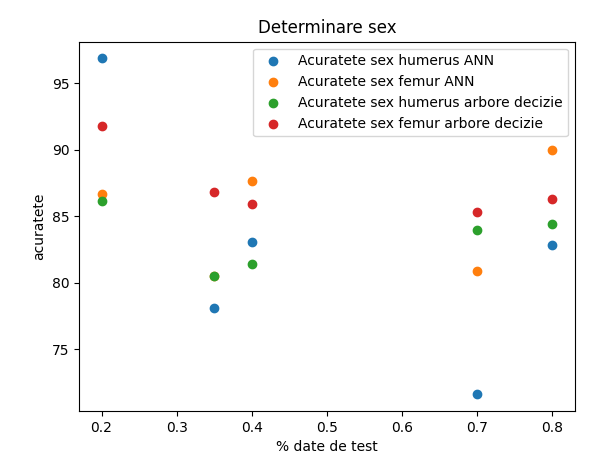
\includegraphics[width=18cm, height=10cm]{Imagini/plot_sex.PNG}
    \caption{Reprezentare grafica a celor doi algoritmi pentru determinarea varstei.}
    \label{plot_age}
\end{figure}

\chapter{Wiki}
\label{chapter:wiki}

Sklearn
\begin{itemize}
    \item \href{https://scikit-learn.org/stable/modules/generated/sklearn.tree.DecisionTreeClassifier.html}{Arbore de decizie}
    \item \href{https://scikit-learn.org/stable/modules/generated/sklearn.metrics.accuracy_score.html}{Acuratete}
    \item \href{https://scikit-learn.org/stable/modules/generated/sklearn.metrics.confusion_matrix.html}{Matrice de confuzie}
    \item \href{https://scikit-learn.org/stable/modules/generated/sklearn.tree.export_graphviz.html}{Vizualizare arbore de decizie}
    \item \href{https://scikit-learn.org/stable/modules/generated/sklearn.tree.export_text.html}{Export arbore de decizie in fisier .dot (decizii ca text)}
    \item \href{https://scikit-learn.org/stable/modules/generated/sklearn.metrics.ConfusionMatrixDisplay.html#sklearn.metrics.ConfusionMatrixDisplay.from_predictions}{Matrice de confuzie}
\end{itemize}

\noindent Keras
\begin{itemize}
    \item \href{https://keras.io/api/models/sequential/}{Structura retelei neuronale}
    \item \href{https://keras.io/api/layers/}{Straturile retelei neuronale}
\end{itemize}

\noindent Citire CSV(Comma Separated Values)
\begin{itemize}
    \item \href{https://pandas.pydata.org/pandas-docs/stable/reference/api/pandas.read_csv.html}{Pandas}
    \item \href{https://docs.python.org/3/library/csv.html}{csv tool}
\end{itemize}

\noindent Set de date
\begin{itemize}
    \item \href{https://web.utk.edu/~auerbach/GOLD.htm}{Goldman Osteometric Data Set}
    \item \href{https://web.utk.edu/~auerbach/GoldMeasures.pdf}{Goldman guide to the measurements}
    \item \href{https://fae.johnshopkins.edu/}{European Data Set-May 2018}
\end{itemize}

\noindent Vizualizare date
\begin{itemize}
    \item \href{https://matplotlib.org/stable/tutorials/introductory/pyplot.html}{Matplotlib}
    \item \href{https://pythonbasics.org/matplotlib-bar-chart/}{Bar chart}
\end{itemize}

\noindent Machine learning
\begin{itemize}
    \item \href{https://en.wikipedia.org/wiki/ID3_algorithm}{Algoritm arbore de decizie articol stiintific mentionat drept referinta}
    \item \href{https://machinelearningmastery.com/classification-and-regression-trees-for-machine-learning/}{Implementare arbori de decizie din sklearn}
    \item \href{https://www.datacamp.com/community/tutorials/decision-tree-classification-python}{Implementare arbori de decizie din sklearn a doua varianta}
\end{itemize}

\noindent Panda3D
\begin{itemize}
    \item \href{https://www.panda3d.org/}{Documentatia oficiala}
\end{itemize}

\noindent Resurse 3D
\begin{itemize}
    \item \href{https://sketchfab.com/3d-models/human-humerus-548132dc5a0a423581e2cba2014ea521}{Model humerus}
    \item \href{https://www.cgtrader.com/items/1020990/download-page}{Model femur}
\end{itemize}

\chapter{Lucrari stiintifice}
\label{chapter:lucrariStiintifice}

Punctul de start al proiectului dat a fost constituit de urmatoarele lucrari stiintifice: \cite{doc1}, \cite{doc2}, \cite{doc3}, \cite{doc4}, \cite{doc5}, \cite{doc6}, \cite{doc7}, \cite{doc8}. Acestea au oferit inspiratia si ajutorul de care am avut nevoie pentru a dezvolta aplicatia. \newline \newline
Pentru implementarea arborelui de decizie si alegerea acestuia in aplicatie s-a folosit lucrarea  \cite{doc7}, de unde am retinut mai ales importanta alegerii unui algoritm care sa fie usor de inteles atat pentru programator, cat si pentru un arheolog pentru a verifica corectitudinea deciziilor. De asemenea, pentru alegerea metricii care selecteaza atributul s-au luat in considerare informatiile prezentate in \cite{doc6}.

\bibliographystyle{plain}
\bibliography{BibAll}

\end{document}

